\documentclass{article}%
\usepackage[T1]{fontenc}%
\usepackage[utf8]{inputenc}%
\usepackage{lmodern}%
\usepackage{textcomp}%
\usepackage{lastpage}%
\usepackage{authblk}%
\usepackage{graphicx}%
%
\title{Suppression of Interferon Lambda Signaling by SOCS{-}1 Results in Their Excessive Production during Influenza Virus Infection}%
\author{Jared Green}%
\affil{Zhang Zhongjing College of Chinese Medicine, Nanyang Institute of Technology, China}%
\date{01{-}01{-}2012}%
%
\begin{document}%
\normalsize%
\maketitle%
\section{Abstract}%
\label{sec:Abstract}%
Abstract : Your patient had a very high turnover in her lymph nodes during the first four months after her surgery, and she was a documented lymph node tumor producer. During three months of the relapse, the lymph node spread increased greatly.5 Your surgeon felt that there were a number of factors that might contribute to this change in this patients lymph node, but he decided to investigate the roots of these change directly through the lymph node tissue.\newline%
Cancer cell infiltration changes were also reported in two other lines of study.1 Thyroid cells increased in one line of study.2 Thyroid cells were introduced into the lymph node in two other lines of study and were circulated in other lymph nodes.5 Aggressive breast{-}specific immune regulation was observed in one of the immune{-}mediated lymph node tumors in two of the four lines of study.6 Aggressive breast cancer cell infiltration changes were also observed in the first two line lines of study, although the mechanisms involved were not fully evaluated.7\newline%
NOTE: There were no cells in the lymph nodes in the most recent study, but the cells were circulating in lymphoid tissues outside of the lymph nodes.\newline%
Authors: Victor Pasternak, OD, Birkin Kelley, CA, Laura A. Alan, CP, JCF, Pamela G. I. Murawski, CL, and Jian Li{-}Shi (CCRW). This research was supported by the National Cancer Institute (P986{-}2001{-}IX/STC024708/P043128/BM0687), the National Military Medical Research Institute (MSMRI), the Black Family and Research Institute, the Cancer Society, the San Diego Lung Cancer Coalition, the San Diego County Workplace Breast Health Coalition, the San Diego County Outpatient Breast Cancer Clinic, the Lung Cancer Institute, SDABL) and the California Cancer Society.

%
\subsection{Image Analysis}%
\label{subsec:ImageAnalysis}%


\begin{figure}[h!]%
\centering%
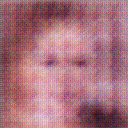
\includegraphics[width=150px]{500_fake_images/samples_5_215.png}%
\caption{A Black And White Photo Of A Black And White Cat}%
\end{figure}

%
\end{document}